\section*{問題1}
${\rm P}\{x_1x_2\leq 0\}=0$であるから,データの取りうる領域は下図の斜線部分(ただし軸上は含まない)のようになる.
\begin{figure}[H]
    \begin{center}
        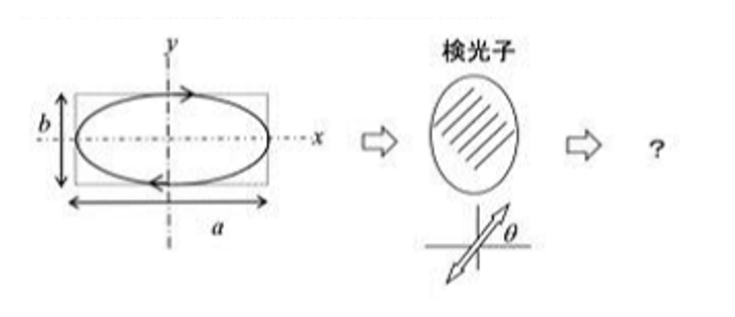
\includegraphics[width=100mm]{./figures/section_1/figure_1.eps}
        \caption{データの取りうる領域}
    \end{center}
\end{figure}
また,${\rm P}\{y=+1|x_1>0\}=1$,${\rm P}\{y=-1|x_2<0\}=1$であるから,正例と負例の現れる領域はそれぞれ下図の斜線部分(ただし軸上は含まない)のようになる.
\begin{figure}[H]
    \begin{minipage}{0.5\hsize}
        \begin{center}
            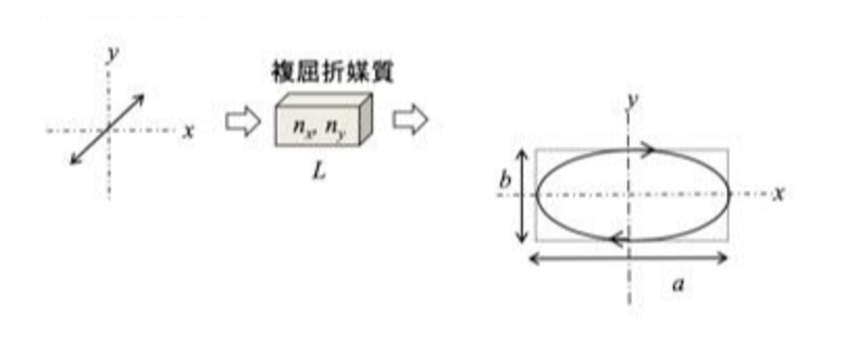
\includegraphics[width=75mm]{./figures/section_1/figure_2.eps}
            \caption{正例の取りうる領域}
        \end{center}
    \end{minipage}
    \begin{minipage}{0.5\hsize}
        \begin{center}
            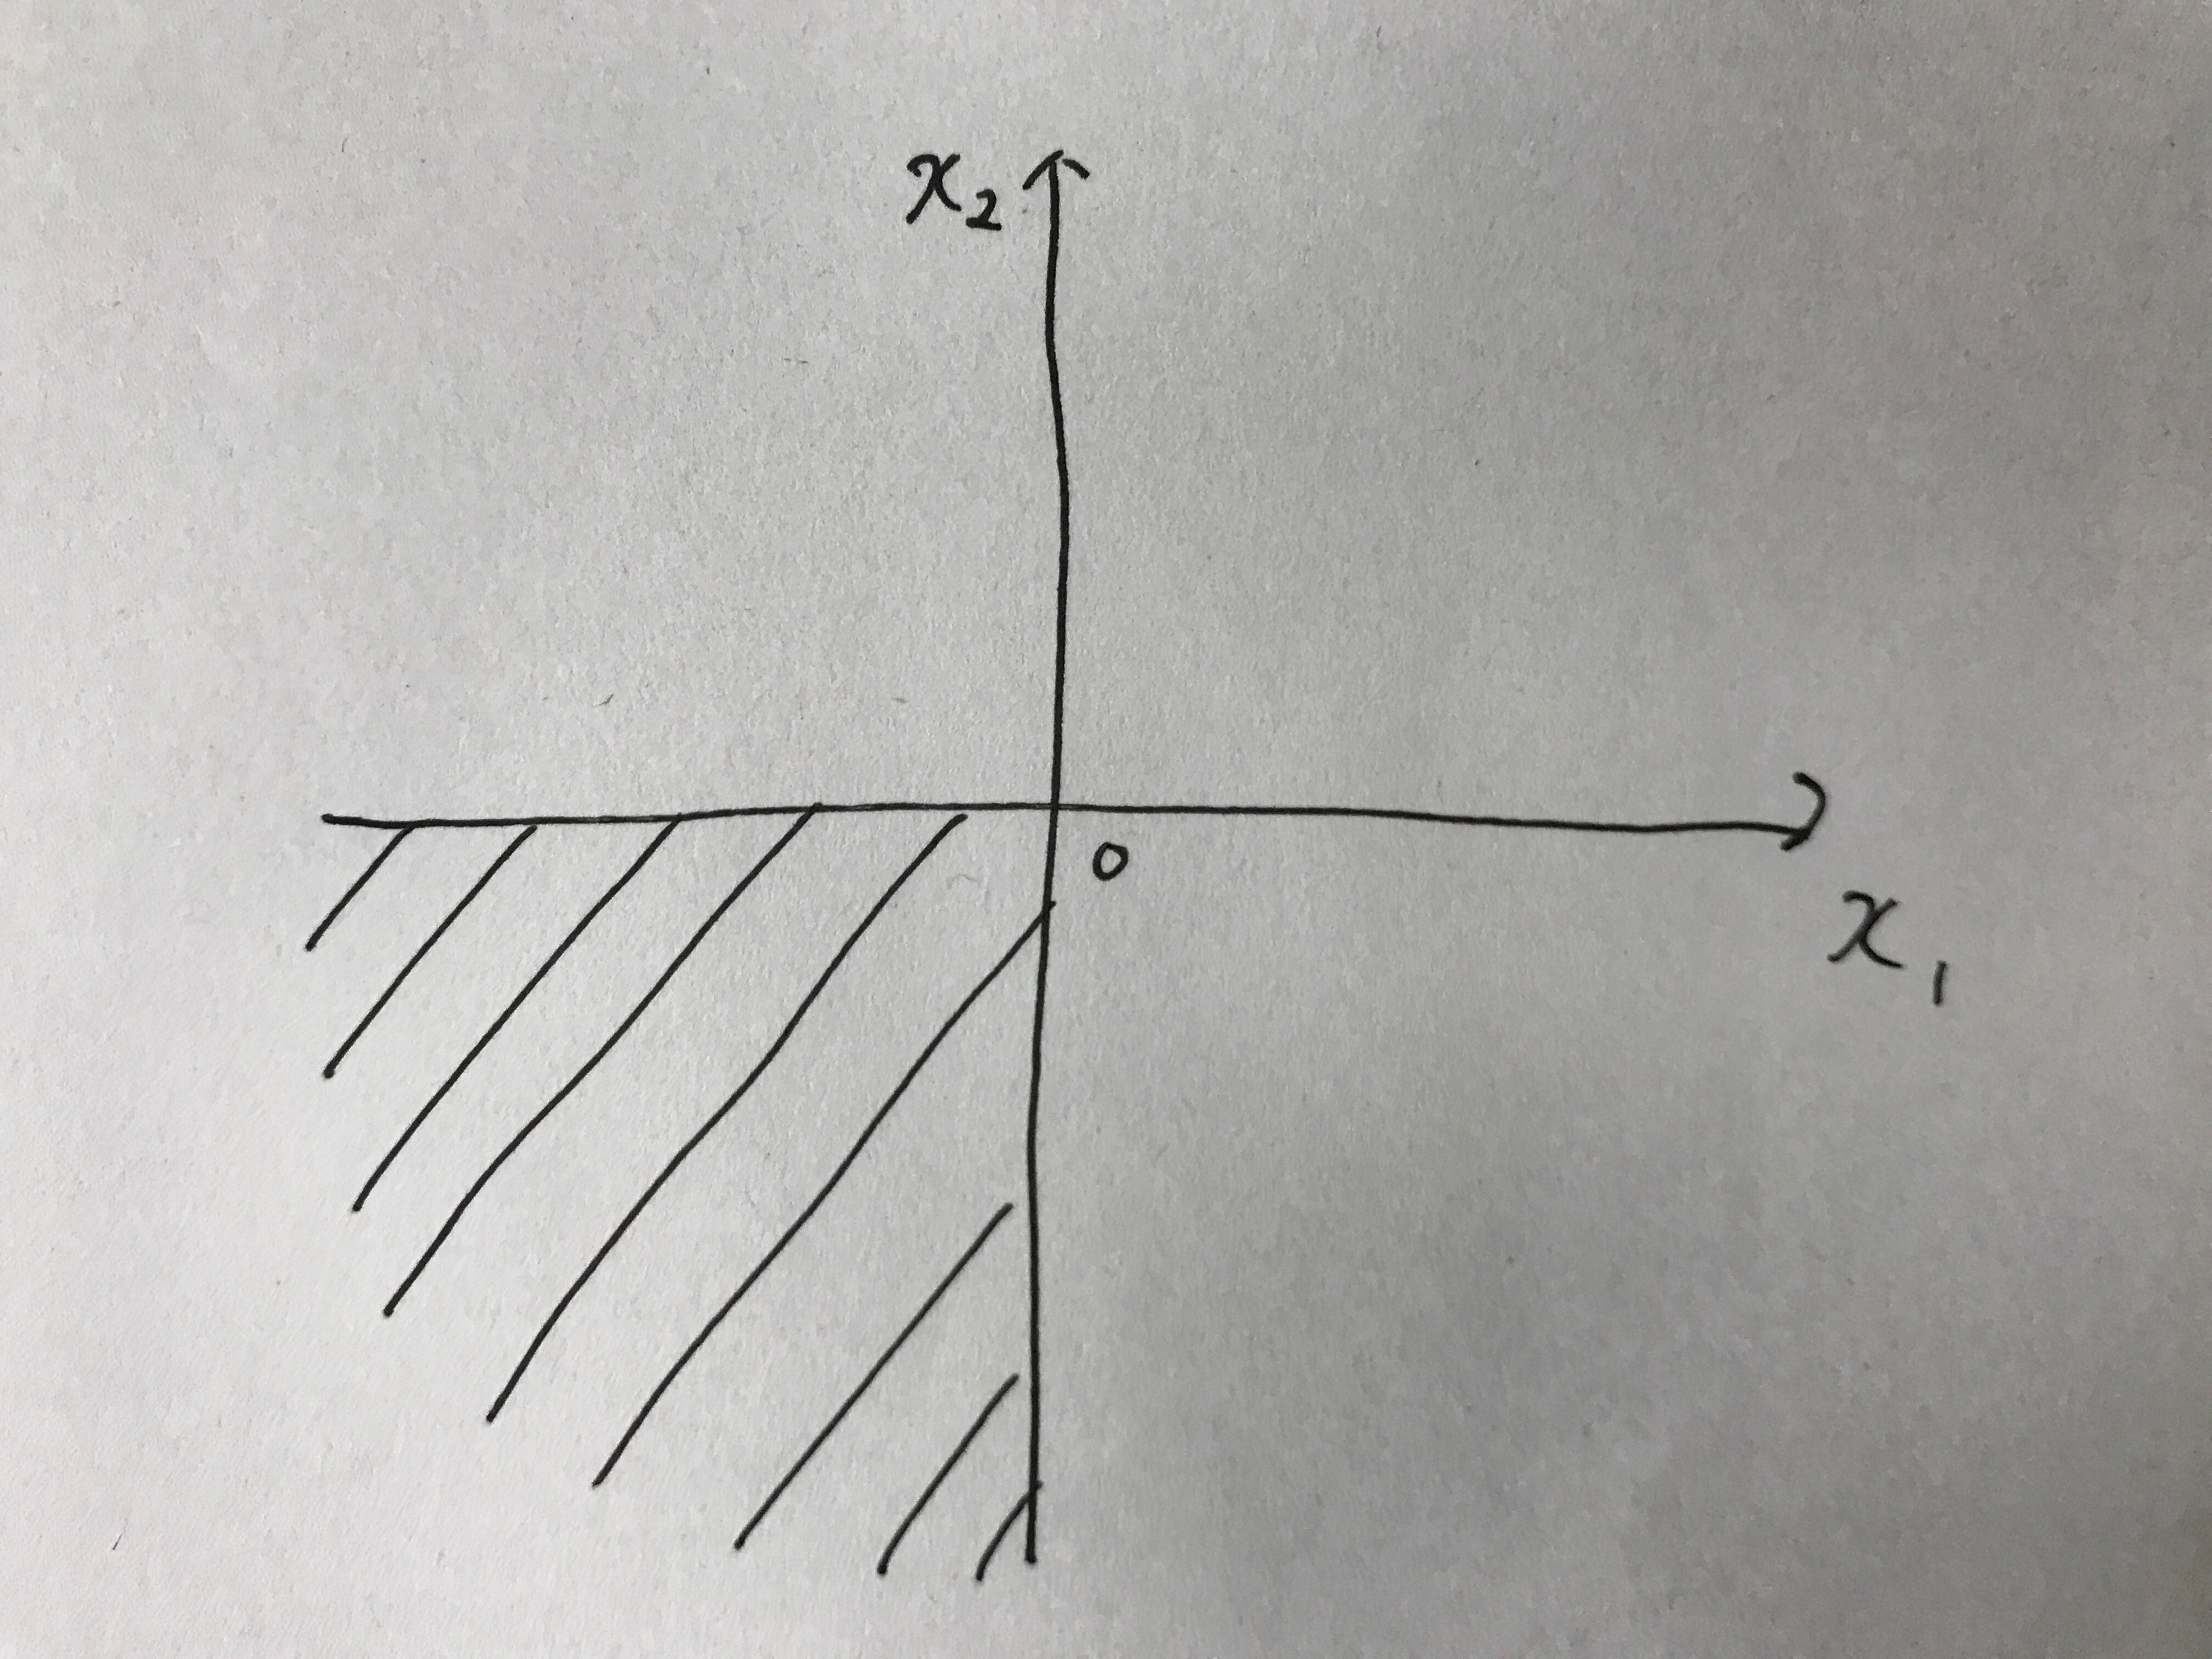
\includegraphics[width=75mm]{./figures/section_1/figure_3.eps}
            \caption{負例の取りうる領域}
        \end{center}
    \end{minipage}
\end{figure}
また,$\bm{\omega}=\left(\begin{array}{c}1\\ 1\end{array}\right)$, $\omega_0=0$とすることで,正例と負例を分離できる.